\documentclass{scrartcl}
\usepackage[utf8]{inputenc}
\usepackage[T1]{fontenc}
\usepackage[english]{babel}
\usepackage{csquotes}
\usepackage[acronym]{glossaries}
\usepackage[binary-units]{siunitx}
\usepackage[backend=biber,style=numeric]{biblatex}
\usepackage[english]{cleveref}
\usepackage[dvipsnames]{xcolor}
\usepackage{subcaption}
\usepackage{pdfpages}
\usepackage{booktabs}
\usepackage{xpatch}
\usepackage[binary-units]{siunitx}
\sisetup{per-mode=symbol}
\DeclareSIUnit{\frm}{frames}
\usepackage{tikz}
\usetikzlibrary{external,calc,positioning,fit,arrows.meta,backgrounds}
\tikzexternalize[prefix=figures/]
\addbibresource{ref.bib}

\title{Partial Reconfiguration of \glsentryshort{fpga} Image Processing
Pipelines with \glsentryshort{pynq}}
\author{Tim Häring}
\date{\today}

% ===============================================
% ===============================================
%     Acronyms
% ===============================================
% ===============================================
% \newacronym{label}{acronym}{description}
\newacronym{aft}{AFT}{Actual Finish Time}
\newacronym{amdovx}{AMDOVX}{AMD OpenVX}
\newacronym{api}{API}{Application Programming Interface}
\newacronym{asic}{ASIC}{Application-specific Integrated Circuit}
\newacronym{ast}{AST}{Actual Start Time}
\newacronym{axi}{AXI}{Advanced eXtensible Interface}
\newacronym{clb}{CLB}{Configurable Logic Block}
\newacronym{cpu}{CPU}{Central Processing Unit}
\newacronym{cu}{CU}{Compute Unit}
\newacronym{cuda}{CUDA}{Compute Unified Device Architecture}
\newacronym{dacc}{DACC}{Dedicated Accelerator}
\newacronym{dag}{DAG}{Directed Acyclic Graph}
\newacronym{dma}{DMA}{Direct Memory Access}
\newacronym{dsl}{DSL}{Domain-specific Language}
\newacronym{dfx}{DFX}{Dynamic Function eXchange}
\newacronym{dsp}{DSP}{Digital Signal Processor}
\newacronym{eft}{EFT}{Earliest Execution Finish Time}
\newacronym{est}{EST}{Earliest Execution Start Time}
\newacronym{ff}{FF}{Flip-Flop}
\newacronym{fifo}{FIFO}{First in, First out}
\newacronym{fpga}{FPGA}{Field Programmable Gate Array}
\newacronym{gdf}{GDF}{Graph Description Format}
\newacronym{gpgpu}{GPGPU}{General-Purpose computing on Graphics Processing Unit}
\newacronym{gpu}{GPU}{Graphics Processing Unit}
\newacronym{hbm}{HBM}{High Bandwidth Memory}
\newacronym{hdl}{HDL}{Hardware Description Language}
\newacronym{heft}{HEFT}{Heterogeneous Earliest Finish Time}
\newacronym{hls}{HLS}{High-Level Synthesis}
\newacronym{hpc}{HPC}{High-Performance Computing}
\newacronym{iacc}{IACC}{Integrated Accelerator}
\newacronym{icd}{ICD}{Installable Client Driver}
\newacronym{ic}{IC}{Integrated Circuit}
\newacronym{ide}{IDE}{Integrated Development Environment}
\newacronym{ii}{II}{Initiation Interval}
\newacronym{ilp}{ILP}{Instruction Level Parallelism}
\newacronym{io}{I/O}{Input/Output}
\newacronym{ip}{IP}{Intellectual Property}
\newacronym{ir}{IR}{Intermediate Representation}
\newacronym{isa}{ISA}{Instruction Set Architecture}
\newacronym{lut}{LUT}{Lookup Table}
\newacronym{mpi}{MPI}{Message Passing Interface}
\newacronym{mpmd}{MPMD}{Multiple Program streams, Multiple Data streams}
\newacronym{msi}{MSI}{Modified/Shared/Invalid}
\newacronym{noc}{NoC}{Network-on-Chip}
\newacronym{oac}{OpenACC}{Open Acceleration}
\newacronym{ocl}{OpenCL}{Open Computing Language}
\newacronym{ocv}{OpenCV}{Open Source Computer Vision Library}
\newacronym{ogl}{OpenGL}{Open Graphics Library}
\newacronym{omp}{OpenMP}{Open Multi-Processing}
\newacronym{os}{OS}{Operating System}
\newacronym{pcie}{PCIe}{Peripheral Component Interconnect Express}
\newacronym{pe}{PE}{Processing Element}
\newacronym{pl}{PL}{Programmable Logic}
\newacronym{ps}{PS}{Processing System}
\newacronym{pynq}{PYNQ}{Python Productivity for Zynq}
\newacronym{ram}{RAM}{Random-Access Memory}
\newacronym{rtl}{RTL}{Register-Transfer Level}
\newacronym{simd}{SIMD}{Single Instruction stream, Multiple Data streams}
\newacronym{slr}{SLR}{Super Logic Region}
\newacronym{soc}{SoC}{System-on-Chip}
\newacronym{tapi}{T-API}{Transparent Application Programming Interface}
\newacronym{tcl}{TCL}{Tool Command Language}
\newacronym{vpu}{VPU}{Vision Processing Unit}
\newacronym{xml}{XML}{Extensible Markup Language}
\newacronym{xrt}{XRT}{Xilinx Runtime}


\begin{document}


\maketitle


\begin{abstract}
This project implements a framework to utilize partial reconfiguration of
\glsentryshortpl{fpga} on a high abstraction level with \glsentryshort{pynq},
which allows software developers to easily benefit from hardware acceleration.
With the help of image processing \glsentryshort{ip}-cores generated with
\glsentryshort{hls}, a prototype algorithm is accelerated by a factor of about
15. The approach using dynamic partial reconfiguration also utilizes only about
half the resources a traditional hardware design would require while offering a
greater amount of functionality, highlighting the benefits of this methodology.
\end{abstract}


\section{Introduction}

Image processing and computer vision have become pervasive in modern society
with applications ranging from robotic vision, object detection and
identification to autonomous driving and many more. With an increasing number of
applications and use cases, the complexity and required computation power of
systems also rose~\cite{kalb2016tulipp}. Many desktop and server applications
are able to use the processing power provided by \glspl{gpu} and countless
frameworks and \glspl{api} are available to ease development, whereas
\glspl{fpga} stood out for applications with tight power constrains and highly
parallel algorithms, though limited by the complexity of the configuration
process~\cite{kalms2017exploration}. This work aims to combine several
approaches that ease \gls{fpga} programming for image processing pipelines with
the help of different abstraction layers and computer vision libraries while
simultaneously overcoming the hard size restrictions that limit the amount of
computation that can be carried out on a \gls{fpga}.


\subsection{Image Processing}

For many years researchers have tried to mimic the human visual system in order
to create robots and digital system with intelligent behaviour. With functions
ranging from facial and gesture recognition to object detection and motion
tracking, the \gls{ocv}~\cite{opencv_library} is one of the most comprehensive
image processing libraries that currently exists. Besides providing several
hundreds of computer vision algorithms, it also allows researchers to easily
experiment and combine different approaches due to its modular structure and
simple \gls{api}. Due to the widespread application of image processing in a
multitude of systems and the similarities of algorithms that operate on video
and image data, this field was chosen to create a proof of concept framework.
With minor tweaks the resulting framework could also be utilized in vastly
different contexts.


\subsection{\glsentryshort{fpga} Programming}

As mentioned previously, creating efficient and correct \gls{fpga} programs is
no simple manner and requires thorough system and device knowledge. Xilinx, one
of the largest manufacturers of \gls{fpga} devices, and many other commercial
vendors, as well as academic researchers, attempted to provide simpler
approaches to hardware programming to open up the possibilities and acceleration
capabilities of these devices to a wider audience~\cite{winterstein2013high}.
\Cref{fig:programming} illustrates different abstraction layers and how they
relate to the traditional programming approach.

\begin{figure}[h]
    \centering
    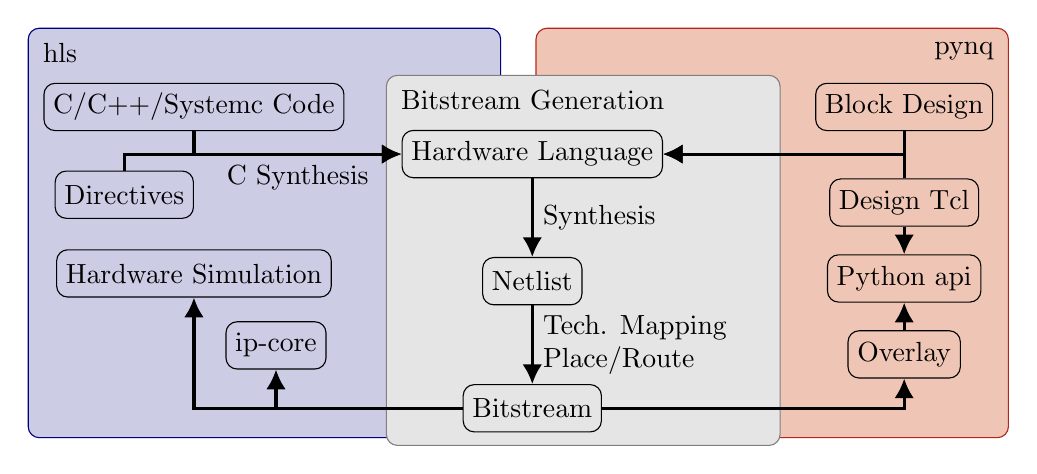
\begin{tikzpicture}
        \tikzset{outer/.style={rounded corners}}
        \tikzset{inner/.style={rounded corners,minimum height=.6cm,draw=black}}
        \tikzset{arr/.style={-{Latex[length=0.25cm,width=0.25cm]},line
        width=.04cm}}

        \node (hls) at (0,0) {};
        \node (hlso) [outer,minimum width=6cm,minimum
            height=5.2cm,fill=NavyBlue!20,draw=NavyBlue] at (hls) {};
        \node (hlsl) [below right=0.1cm of hlso.north west]
            {\glsentrylong{hls}};
        \node (hls0) [inner,below right=0.7cm and 0.2cm of hlso.north west]
            {C/C++/Systemc Code};
        \node (hls1) [inner,below left=0.5cm and 0cm of hls0.south]
            {Directives};
        \node (hls2) [inner,below=1.5cm of hls0] {Hardware Simulation};
        \node (hls3) [inner,below right=0.3cm and 0.4cm of hls2.south]
            {\glsentryshort{ip}-core};

        \node (pynq) [right=6.2cm of hls] {};
        \node (pynqo) [outer,minimum width=6cm,minimum
            height=5.2cm,fill=BrickRed!20,draw=BrickRed] at (pynq) {};
        \node (pynql) [below left=0.1cm of pynqo.north east]
            {\glsentrylong{pynq}};
        \node (pynq0) [inner,below left=0.7cm and 0.2cm of pynqo.north east]
            {Block Design};
        \node (pynq1) [inner,below=0.6cm of pynq0.south] {Design Tcl};
        \node (pynq2) [inner,below=0.35cm of pynq1.south] {Python \gls{api}};
        \node (pynq3) [inner,below=0.35cm of pynq2.south] {Overlay};

        \node (bs) [below right=0.1cm and 3.8cm of hls] {};
        \node (bso) [outer,minimum width=5cm,minimum
            height=4.7cm,fill=Gray!20,draw=Gray] at (bs) {};
        \node (bsl) [below right=0.1cm of bso.north west] {Bitstream
            Generation};
        \node (bs0) [inner,below right=0.7cm and 0.2cm of bso.north west]
            {Hardware Language};
        \node (bs1) [inner,below=1cm of bs0] {Netlist};
        \node (bs2) [inner,below=1cm of bs1] {Bitstream};

        \draw [arr] let \p1 = (hls0.south), \p2 = (bs0.west) in (\x1,\y1) --
            (\x1,\y2) -- node [below] {C Synthesis} (\x2,\y2);
        \draw [arr] let \p1 = (hls1.north), \p2 = (bs0.west) in (\x1,\y1) --
            (\x1,\y2) -- (\x2,\y2);
        \draw [arr] let \p1 = (bs2.west), \p2 = (hls2.south) in (\x1,\y1) --
            (\x2,\y1) -- (\x2,\y2);
        \draw [arr] let \p1 = (bs2.west), \p2 = (hls3.south) in (\x1,\y1) --
            (\x2,\y1) -- (\x2,\y2);

        \draw [arr] let \p1 = (pynq0.south), \p2 = (bs0.east) in (\x1,\y1) --
            (\x1,\y2) -- (\x2,\y2);
        \draw [arr] let \p1 = (pynq1.north), \p2 = (bs0.east) in (\x1,\y1) --
            (\x1,\y2) -- (\x2,\y2);
        \draw [arr] let \p1 = (bs2.east), \p2 = (pynq3.south) in (\x1,\y1) --
            (\x2,\y1) -- (\x2,\y2);
        \draw [arr] (pynq3) -- (pynq2);
        \draw [arr] (pynq1) -- (pynq2);

        \draw [arr] (bs0) -- node [right] {Synthesis} (bs1);
        \draw [arr] (bs1) -- node [right,align=left] {Tech.
        Mapping\\Place/Route} (bs2);
    \end{tikzpicture}
    \caption{Different \gls{fpga} programming abstraction layers.}%
    \label{fig:programming}%
\end{figure}

While the conventional approach of bitstream generation requires users to define
the hardware they would like to create in a \gls{hdl}, \gls{hls} and \gls{pynq}
provide abstraction layers in high-level languages that are familiar to software
developers.


\subsubsection{\glsentrylong{hls}}

Using \gls{hls} for \gls{fpga} development allows for easier and faster testing
of functional correctness, portability of code and shorter development cycles.
Vivado \gls{hls} from Xilinx uses pragmas to annotate C/C++/SystemC code with
compiler hints in order to produce efficient hardware. This way developers do
not need to learn a \gls{hdl} or \gls{dsl} but creating complex systems still
requires profound knowledge of the underlying hardware. Because of the huge
popularity and wide spread usage of the \gls{ocv} library, Xilinx provides an
equivalent \gls{hls} implementation of most of the functionality annotated with
appropriate pragmas to produce effective circuits, which was used throughout the
curse of this project.


\subsubsection{\glsentrylong{pynq}}

\gls{pynq} provides software developers the opportunity to easily access and
utilize custom circuit functionality and to collaborate closer with hardware
engineers. It allows for re-usage of carefully crafted hardware definitions
through an abstract and simple Python \gls{api}. It can only be used on the
Xilinx systems that combine a \gls{ps} and \gls{pl} into one \gls{soc}. The
\gls{ps} runs a custom Linux operating system that provides a Jupyter-Notebook
server for quick and easy access to the system. Python is then used to control
the \gls{ps} and perform calculations in software, as well as to specify the
hardware building blocks and delegate computation to the custom circuits
implemented by the selected overlay. With this dynamic approach, computation
offloading can be easily tested and evaluated without any hardware development
knowledge.


\subsubsection{Partial Reconfiguration}

Where \glspl{cpu} and \glspl{gpu} can simply be tasked to carry out specific
calculations by executing machine code, \glspl{fpga} can only ever execute the
algorithms that were synthesized to the bitstream that was used to program the
device. Since the amount of reconfigurable elements on an \gls{fpga} is limited,
this poses a hard limit to the number of accelerators that can be executed on
the \gls{fpga}. When another functionality is required, the entire \gls{fpga}
needs to be reconfigured with a new bitstream that needs to be synthesized
first. As bitstream creation (one hour or more) and \gls{fpga} reconfiguration
(several seconds or more) is very costly time wise, even live reconfiguration is
not feasible in an image processing context. To circumvent this limitation,
Xilinx provides \gls{dfx}, which allows for the reconfiguration of modules
within an active design. \Cref{fig:reconf} illustrates this behaviour.

\begin{figure}[h]
    \centering
    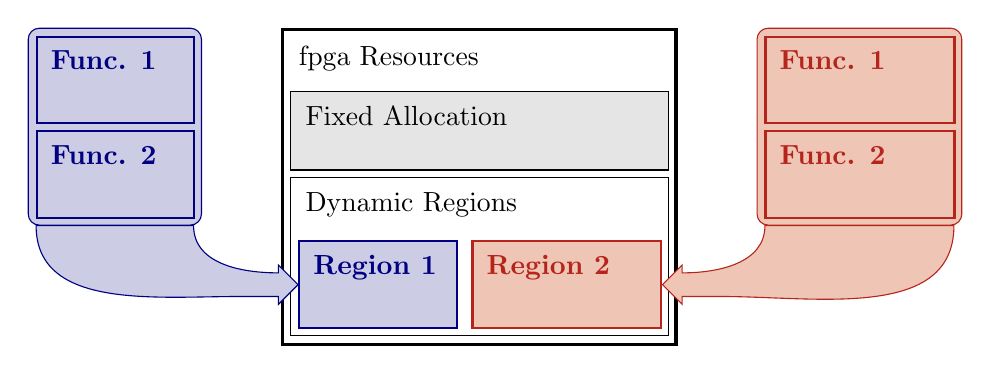
\begin{tikzpicture}
        \tikzset{dfx2/.style={minimum width=2.4cm,minimum
            height=1.1cm,fill=BrickRed!20,draw=BrickRed,thick}}
        \tikzset{dfx1/.style={minimum width=2.0cm,minimum
            height=1.1cm,fill=NavyBlue!20,draw=NavyBlue,thick}}
        \node (res) at (0,0) [draw,very thick,minimum width=5cm,minimum
            height=4cm] {};
        \node (resl) [below right=0.15cm of res.north west] {\gls{fpga}
            Resources};
        \node (fix) [draw,below right=0.8cm and 0.12cm of res.north west,minimum
            width=4.8cm,minimum height=1cm,fill=Gray!20] {};
        \node (fixl) [below right=0.1cm of fix.north west] {Fixed Allocation};
        \node (dyn) [draw,below right=1.9cm and 0.12cm of res.north west,minimum
            width=4.8cm,minimum height=2cm] {};
        \node (dynl) [below right=0.1cm of dyn.north west] {Dynamic Regions};
        \node (r1) [below right=0.8cm and 0.1cm of dyn.north west,dfx1] {};
        \node (r1l) [below right=0.1cm of r1.north west,color=NavyBlue]
            {\textbf{Region 1}};
        \node (r2) [below right=0.8cm and 2.3cm of dyn.north west,dfx2] {};
        \node (r2l) [below right=0.1cm of r2.north west,color=BrickRed]
            {\textbf{Region 2}};

        \node (pr1) [below left=0cm and 1cm of res.north west,minimum
            width=2.2cm,minimum
            height=2.5cm,fill=NavyBlue!20,draw=NavyBlue,rounded corners] {};
        \node (pr1f1) [below right=0.1cm and 0.1cm of pr1.north west,dfx1] {};
        \node (pr1f1l) [below right=0.1cm of pr1f1.north west,color=NavyBlue]
            {\textbf{Func. 1}};
        \node (pr1f2) [below right=1.3cm and 0.1cm of pr1.north west,dfx1] {};
        \node (pr1f2l) [below right=0.1cm of pr1f2.north west,color=NavyBlue]
            {\textbf{Func. 2}};

        \node (pr2) [below right=0cm and 1cm of res.north east,minimum
            width=2.6cm,minimum
            height=2.5cm,fill=BrickRed!20,draw=BrickRed,rounded corners] {};
        \node (pr2f1) [below right=0.1cm and 0.1cm of pr2.north west,dfx2] {};
        \node (pr2f1l) [below right=0.1cm of pr2f1.north west,color=BrickRed]
            {\textbf{Func. 1}};
        \node (pr2f2) [below right=1.3cm and 0.1cm of pr2.north west,dfx2] {};
        \node (pr2f2l) [below right=0.1cm of pr2f2.north west,color=BrickRed]
            {\textbf{Func. 2}};

        \filldraw [fill=NavyBlue!20,draw=NavyBlue] let \p1 = (pr1.south), \p2 =
            (r1.west) in (\x2,\y2) -- ++(-0.25,-0.25) -- ++(0,0.1) -- ++(-0.5,0)
            to [out=180,in=270] (\x1 - 1cm,\y1) -- (\x1 + 1cm,\y1) to
            [out=270,in=180] (\x2 - 0.25cm, \y2 + 0.15cm) -- ++(0,0.1) -- cycle;

        \filldraw [fill=BrickRed!20,draw=BrickRed] let \p1 = (pr2.south), \p2 =
            (r2.east) in (\x2,\y2) -- ++(0.25,-0.25) -- ++(0,0.1) -- ++(0.5,0)
            to [out=0,in=270] (\x1 + 1.2cm,\y1) -- (\x1 - 1.2cm,\y1) to
            [out=270,in=0] (\x2 + 0.25cm, \y2 + 0.15cm) -- ++(0,0.1) -- cycle;
    \end{tikzpicture}
    \caption{\gls{fpga} resource usage with partial reconfiguration.}%
    \label{fig:reconf}%
\end{figure}

While not being able to completely negate the downside of limited reprogrammable
fabric, partial reconfiguration offers several advantages. As stated
in~\cite{kao2005benefits}, it allows for increased system performance since
swapping functionality does not require downtime, hardware sharing for reduced
power consumption and cost, and shorter reconfiguration times since the partial
bitstreams are smaller.


\section{Motivation and Related Work}

There exists a lot of work on the topic of partial reconfiguration: the authors
of~\cite{lie2009dynamic} explore the resulting reconfiguration time and
bitstream size and simply provide evidence for the claims made
in~\cite{kao2005benefits}. The paper~\cite{liu2009run} follows in a similar
vein, but additionally proposes to utilize Block \gls{ram} to reconfigure
regions even quicker but at the cost of increased resource utilization.
In~\cite{beckhoff2012go} the authors introduce a framework to automate aspects
of the processes required to implement partial reconfiguration on Xilinx
devices, a feature which is natively covered almost completely by the Xilinx
Vivado tool nowadays. This means, partial reconfiguration can be used quite
easily by hardware developers, but there is no simplified way to create a
bitstream that supports it through \gls{hls} or \gls{pynq}. The goal of this
project is to create a framework that enables software developers to utilize
dynamic partial reconfiguration and hardware acceleration through the simple and
familiar Python programming language. As a proof of concept, an image processing
pipeline with different regions and dynamic functions was implemented.


\section{Partial Reconfiguration of Image Processing Pipelines}

The framework consist of several components, the overall approach is depicted in
\Cref{fig:approach}.

\begin{figure}[h]
    \centering
    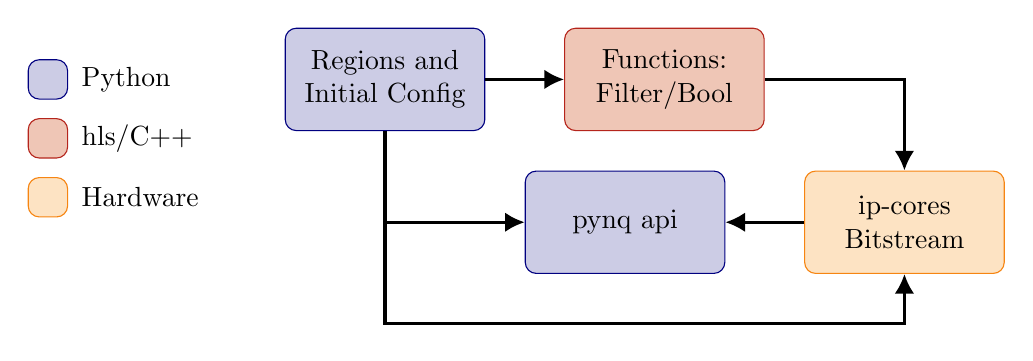
\begin{tikzpicture}
        \tikzset{node/.style={rounded corners,minimum
            height=1.3cm,align=center,text width=2.3cm}}
        \tikzset{leg/.style={rounded corners,minimum
            height=0.5cm,minimum width=0.5cm}}
        \tikzset{python/.style={fill=NavyBlue!20,draw=NavyBlue,node}}
        \tikzset{hls/.style={fill=BrickRed!20,draw=BrickRed,node}}
        \tikzset{ip/.style={fill=BurntOrange!20,draw=BurntOrange,node}}
        \tikzset{pythonl/.style={fill=NavyBlue!20,draw=NavyBlue,leg}}
        \tikzset{hlsl/.style={fill=BrickRed!20,draw=BrickRed,leg}}
        \tikzset{ipl/.style={fill=BurntOrange!20,draw=BurntOrange,leg}}
        \tikzset{arr/.style={-{Latex[length=0.25cm,width=0.25cm]},line
            width=.04cm}}

        \node (p) at (0,0) [python] {Regions and\\Initial Config};
        \node (h) [right=of p,hls] {Functions:\\Filter/Bool};
        \node (i) [below right=0.5cm and 0.5cm of h,ip]
            {\glsentryshort{ip}-cores\\Bitstream};
        \node (pynq) [below right=0.5cm and 0.5cm of p,python] {\gls{pynq}
            \gls{api}};
        \node (help) [below=0.5cm of i] {};

        \node (legp) at (-4,0) {};
        \node [left=-0.1cm of legp,pythonl] {};
        \node [right=-0.1cm of legp] {Python};
        \node (legh) [below=0.5cm of legp] {};
        \node [left=-0.1cm of legh,hlsl] {};
        \node [right=-0.1cm of legh] {\gls{hls}/C++};
        \node (legi) [below=0.5cm of legh] {};
        \node [left=-0.1cm of legi,ipl] {};
        \node [right=-0.1cm of legi] {Hardware};

        \draw [arr] (p.south) |- (pynq.west);
        \draw [arr] (p.east) -- (h.west);
        \draw [arr] (h.east) -| (i.north);
        \draw [arr] (i.west) -- (pynq.east);
        \draw [arr] let \p1 = (p.south), \p2 = (help), \p3 = (i.south) in
            (\x1,\y1) -- (\x1,\y2) -- (\x2,\y2) -- (\x3,\y3);
    \end{tikzpicture}
    \caption{Framework components overview.}%
    \label{fig:approach}%
\end{figure}

A Python script on the development PC holds information about the available
functions and the initial configuration of all regions. All available functions
were previously implemented using \gls{hls} and the Xilinx \gls{ocv} library
\texttt{xfOpenCV}, which allows for simple generation of hardware. Only the
function interfaces need to be explicitly defined, everything else is analog to
a software development process. The Python script calls the Vivado \gls{hls}
compiler, which creates \gls{ip}-cores for all defined functions where the
target clock frequency and target platform can be set. Afterwards, a base design
for the selected platform is created with the Vivado tool in batch mode. Then
the design is configured for dynamic partial reconfiguration and the regions and
constraints are set accordingly. The resulting bitstreams and \texttt{.tcl}
files can then be used to program the \gls{fpga} from within the \gls{pynq}
environment running on the \gls{soc}. After programming the \gls{fpga}, the
individual accelerators can be utilized to increase the performance of the
application.


\subsection{\glsentrylong{ps}}

The prototype image processing pipeline that was implemented consists of the
functions depicted in \Cref{fig:func}.

\begin{figure}[h]
    \centering
    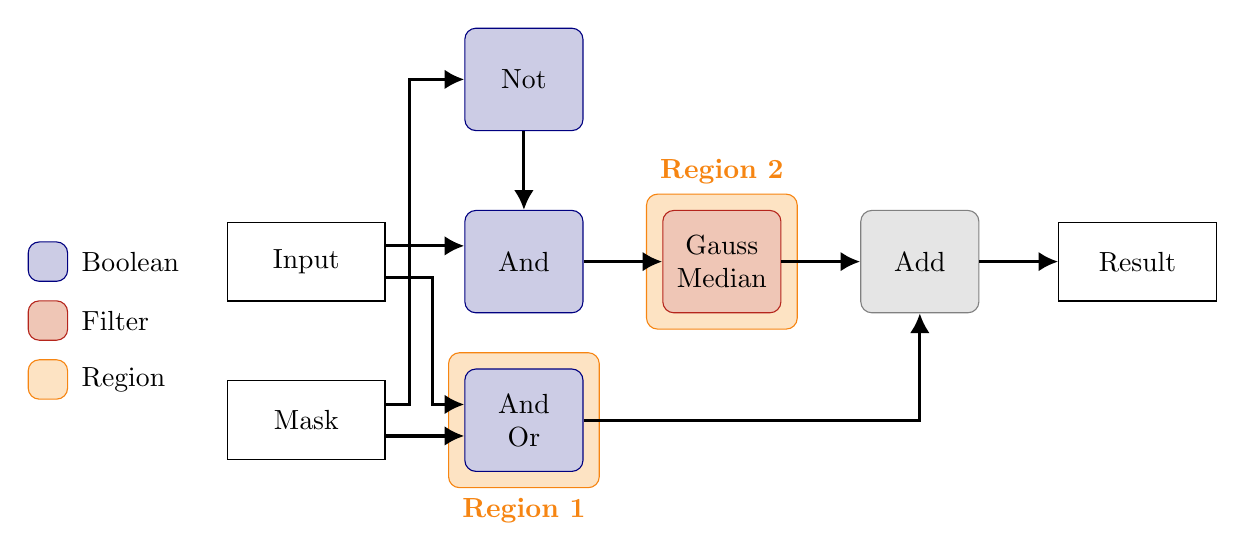
\begin{tikzpicture}
        \tikzset{img/.style={draw,minimum width=2.0cm,minimum height=1.0cm}}
        \tikzset{node/.style={rounded corners,minimum width=1.5cm,minimum
            height=1.3cm,align=center}}
        \tikzset{reg/.style={rounded corners,inner sep=0.2cm}}
        \tikzset{leg/.style={rounded corners,minimum width=0.5cm,minimum
            height=0.5cm}}
        \tikzset{bool/.style={fill=NavyBlue!20,draw=NavyBlue,node}}
        \tikzset{addn/.style={fill=Gray!20,draw=Gray,node}}
        \tikzset{filter/.style={fill=BrickRed!20,draw=BrickRed,node}}
        \tikzset{region/.style={fill=BurntOrange!20,draw=BurntOrange,reg}}
        \tikzset{booll/.style={fill=NavyBlue!20,draw=NavyBlue,leg}}
        \tikzset{filterl/.style={fill=BrickRed!20,draw=BrickRed,leg}}
        \tikzset{regionl/.style={fill=BurntOrange!20,draw=BurntOrange,leg}}
        \tikzset{arr/.style={-{Latex[length=0.25cm,width=0.25cm]},line
            width=.04cm}}

        \node (input) at (0,0) [img] {Input};
        \node (mask) [below=of input,img] {Mask};
        \node (bool1) [right=of mask,bool] {And\\Or};
        \node (bool2) [right=of input,bool] {And};
        \node (not) [above=of bool2,bool] {Not};
        \node (filter) [right=of bool2,filter] {Gauss\\Median};
        \node (add) [right=of filter,draw,addn] {Add};
        \node (res) [right=of add,img] {Result};

        \node (legb) at (-3,0) {};
        \node [left=-0.1cm of legb,booll] {};
        \node [right=-0.1cm of legb] {Boolean};
        \node (legf) [below=0.5cm of legb] {};
        \node [left=-0.1cm of legf,filterl] {};
        \node [right=-0.1cm of legf] {Filter};
        \node (legr) [below=0.5cm of legf] {};
        \node [left=-0.1cm of legr,regionl] {};
        \node [right=-0.1cm of legr] {Region};

        \begin{scope}[on background layer]
            \node (r1) [region,fit=(bool1)] {};
            \node [below=0cm of r1,color=BurntOrange] {\textbf{Region 1}};
            \node (r2) [region,fit=(filter)] {};
            \node [above=0cm of r2,color=BurntOrange] {\textbf{Region 2}};
        \end{scope}

        \draw [arr] let \p1 = (input.east), \p2 = (bool1.west) in
            (\x1,\y1-0.2cm) -- ++(0.6cm,0) |- (\x2,\y2+0.2cm);
        \draw [arr] let \p1 = (mask.east), \p2 = (bool1.west) in (\x1,\y1-0.2cm)
            -- (\x2,\y2-0.2cm);
        \draw [arr] let \p1 = (mask.east), \p2 = (not.west) in (\x1,\y1+0.2cm)
            -- ++(0.3cm,0) |- (\x2,\y2);
        \draw [arr] (not.south) -- (bool2.north);
        \draw [arr] let \p1 = (input.east), \p2 = (bool2.west) in
            (\x1,\y1+0.2cm) -- (\x2,\y2+0.2cm);
        \draw [arr] (bool2.east) -- (filter.west);
        \draw [arr] (filter.east) -- (add.west);
        \draw [arr] (bool1.east) -| (add.south);
        \draw [arr] (add.east) -- (res.west);
    \end{tikzpicture}
    \caption{Implemented prototype algorithm.}%
    \label{fig:func}%
\end{figure}

While the pipeline consists of multiple functions, only the boolean functions
“And” and “Or” and the filter functions “Gauss” and “Median” were implemented as
dynamic partial regions with two different functions that can be inserted in
each region respectively. The input and resulting images are shown in
\Cref{fig:images}.

\begin{figure}[h]
    \centering
    \begin{subfigure}{.3\textwidth}
        \centering
        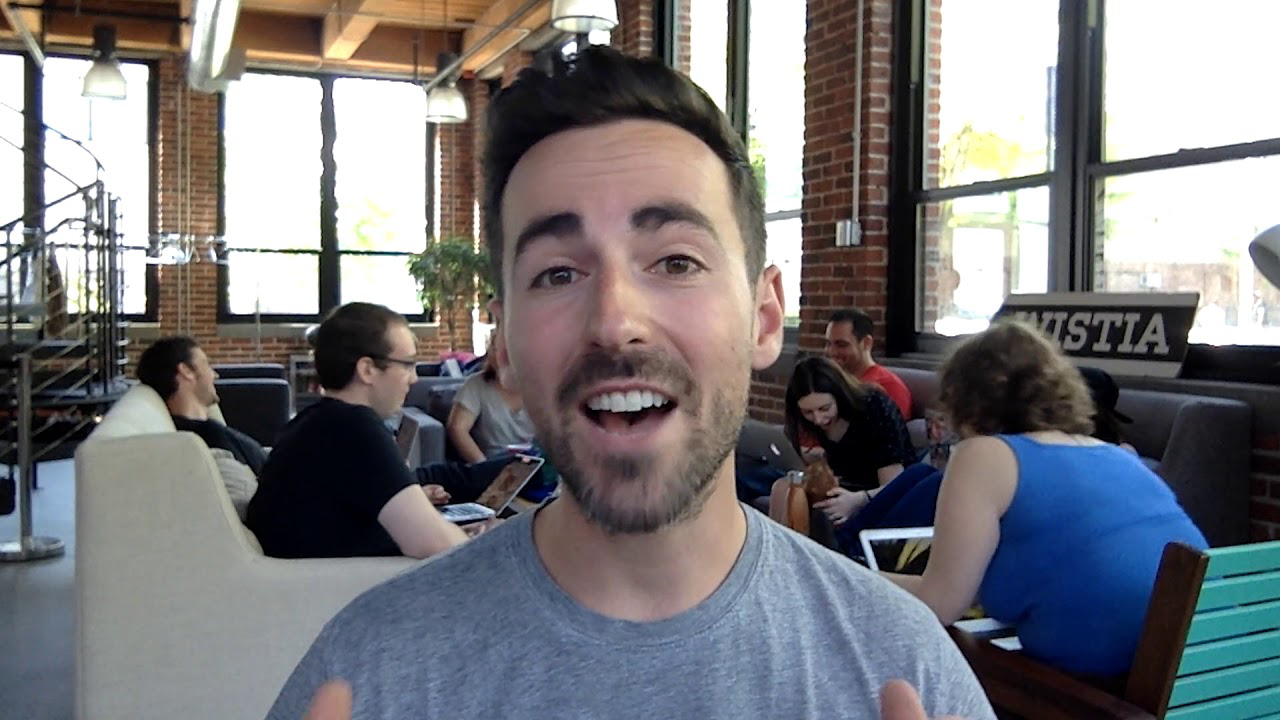
\includegraphics[width=\linewidth]{../../python/person}
        \subcaption{Input Image}%
        \label{subfig:input}
    \end{subfigure}\hfill
    \begin{subfigure}{.3\textwidth}
        \centering
        
\includegraphics[width=\linewidth]{../../python/and_gauss_81}
        \subcaption{And/Gauss}%
        \label{subfig:input}
    \end{subfigure}\hfill
    \begin{subfigure}{.3\textwidth}
        \centering
        
\includegraphics[width=\linewidth]{../../python/and_median_81}
        \subcaption{And/Median}%
        \label{subfig:input}
    \end{subfigure}\hfill
    \medskip
    \begin{subfigure}{.3\textwidth}
        \centering
        
\includegraphics[width=\linewidth]{../../python/mask_big}
        \subcaption{Mask}%
        \label{subfig:input}
    \end{subfigure}\hfill
    \begin{subfigure}{.3\textwidth}
        \centering
        
\includegraphics[width=\linewidth]{../../python/or_gauss_81}
        \subcaption{Or/Gauss}%
        \label{subfig:input}
    \end{subfigure}\hfill
    \begin{subfigure}{.3\textwidth}
        \centering
        
\includegraphics[width=\linewidth]{../../python/or_median_81}
        \subcaption{Or/Median}%
        \label{subfig:input}
    \end{subfigure}\hfill
    \caption{Inputs and results of the image processing pipeline.}%
    \label{fig:images}%
\end{figure}

To amplify the filter results, the kernel size was set to $81 \times 81$ but
only to produce these showcase images. To obtain the performance results the
kernel size was set to $3 \times 3$ for both the hardware and the software
implementation. The characteristics of the different filters clearly show in the
results. While the combination of the boolean “And” and both filters produces
an image that could be used in a real world application, the “Or” operation does
not produce any useful results and was only used to demonstrate the partial
reconfiguration capabilities of the processing pipeline.


\subsection{\glsentrylong{pl}}

Three overlays were created throughout the course of this project:

\begin{itemize}
    \item Base: this bitstream contains two of the four possible pipelines,
        namely the combination “And” and “Median”, as well as the “Or” and
        “Gauss” pipeline. This serves as comparison for the design that
        implements the partial reconfiguration with regards to resource
        utilization.
    \item Streaming: similar to the base bitstream but only implements one
        pipeline. Instead of going through the \gls{ps} \gls{ram}, the HDMI
        video streams are entirely processed on the \gls{pl}. The \gls{pynq}
        \gls{api} is only used to start the processing and does not interact
        with the \gls{pl} during runtime. This serves as another data point when
        comparing the resulting performance.
    \item Partial: this bitstream implements the algorithmic depiction of the
        pipeline as given in \Cref{fig:func}. The entire design and all aspects
        of partial reconfiguration were automatically created by the Python and
        \texttt{.tcl} build scripts.
\end{itemize}

In the “Base” and “Partial” designs, the data transfers happen through \gls{axi}
streaming interfaces that communicate with the \gls{ram} of the development
board. To execute the pipelines and utilize the partial reconfiguration, the
hardware has to be programmed with the static part of the partial bitstream and
the desired functions for each region from within the \gls{pynq} environment.
Afterwards, the Python wrapper for an \gls{axi} \gls{dma} is used to send the
images from the \gls{ram} to the acceleration cores and read the result back
into memory.


\section{Evaluation and Results}

All designs were created using the 2021.1 version of the Vivado tool, since this
is the first version that supports partial reconfiguration when working with a
block design. Only one clock set to \SI{100}{\mega\hertz} was used in the
entire design. The measurements were conducted with full HD images with three
data channels, which results in about \SI{2}{\mega\byte} per image. To obtain
results for the frames-per-second measurements, each filter was run \num{100}
times and the resulting duration was used to calculate the metric.


\subsection{Resource Utilization}

Since hardware resources within a \gls{fpga} are limited, a more space-efficient
design is able to achieve greater flexibility and function range.
\Cref{tab:res} gives an overview of the resource utilization percentage of the
implemented overlays.

\begin{table}[h]
    \centering
    \begin{tabular}{l S S S}
        \toprule
        {Overlay} & {Slice \glsentryshort{lut}}\ [\si{\percent}] &
        {B\glsentryshort{ram}}\ [\si{\percent}] & {\glsentryshort{dsp}}\
        [\si{\percent}] \\
        \midrule
        Base        & 54.52 &  9.29 & 35.45 \\
        Streaming   & 62.43 & 16.43 & 12.18 \\
        Partial     & 31.78 &  5.36 & 10.91 \\
        \bottomrule
    \end{tabular}
    \caption{Resource utilization percentage of the implemented overlays.}%
    \label{tab:res}%
\end{table}

The “Base” overlay contains two parallel pipelines and thus uses more resources
than the “Partial” overlay. This is expected but it also clearly shows the
advantages of dynamic partial reconfiguration. Even with the increased resource
utilization, the “Base” overlay is not able to fully replicate the functionality
of the “Partial” overlay, the combinations “Or” and “Median”, as well as “And”
and “Gauss” are missing. This feature disparity will only increase with a
growing number of regions and functions available in the block design with
partial reconfiguration. The “Streaming” overlay uses even more resources since
it also needs to accommodate various \gls{ip}-cores for raw HDMI signal handling
and processing. This overlay does not need to utilize the \gls{ps} \gls{ram} and
thus the performance is slightly better as the next section will show.
Integrating partial reconfiguration into this design would also be possible, but
was not done during this project due to time constraints. However, it would have
been a good fit since the resources are already used quite heavily and adding
further functionality not only increases the bitstream generation time but is
also increasingly likely to fail since the synthesis tool is not able to create
a hardware implementation that meets the required timings.


\subsection{Performance}

Another important aspect of creating a hardware/software co-design is the
resulting performance of the system. \Cref{tab:perf} shows the latency and
calculated frames-per-second metric of the \gls{ps} and \gls{pl} execution
respectively.

\begin{table}[h]
    \centering
    \begin{tabular}{l S S}
        \toprule
        Overlay & {Latency}\ [\si{\milli\second}] & {Performance}\
        [\si{\frm\per\second}] \\
        \midrule
        Base        &  22.73 & 43.98 \\
        Streaming   &  20.83 & 48.00 \\
        Partial     &  23.35 & 42.82 \\
        \midrule
        Software    & 365.03 &  2.73 \\
        \bottomrule
    \end{tabular}
    \caption{Performance results of different implementations.}%
    \label{tab:perf}%
\end{table}

All implementations execute the algorithm depicted in \Cref{fig:func} with the
“And” and “Median” function selected, the “Base” overlay also computes the “Or”
and “Gauss” pipeline but in parallel, so this should not add to the resulting
execution time. Those measurements clearly show the advantages of hardware
acceleration in this context, all hardware implementations are about 15 times
faster than the execution in software. Unfortunately, all designs are not able
to achieve a frame rate of \SI{60}{\frm\per\second}, but this is expected
behaviour since the amount of pixels in a full HD image is about \num{2} million
which is equivalent to the amount of required clock cycles. This results in an
optimal execution time of \SI{20.736}{\milli\second}, which the “Streaming”
overlay is almost able to achieve. Some additional clock cycles are required to
fill the intermediate \gls{fifo} buffers and processing pipelines within the
individual functions. Since the “Base” and “Partial” overlay use an \gls{axi}
\gls{dma} to transfer the data from and to the main memory, some additional
delays were introduced. Although the specification of the
memory~\cite{pynqz1spec} indicates that it would support bandwidths of about
\SI{131.25}{\mega\byte\per\second}, which would result in approximately
\SI{66}{\frm\per\second}, the additional delay of the \gls{axi} \gls{dma} limits
this to the results obtained in \Cref{tab:perf}.


\section{Conclusion and Outlook}

In this project an image processing framework prototype has been implemented.
The framework is able to create computer vision pipelines with arbitrary
building blocks after they were defined using \gls{hls} and connected as given
in \Cref{fig:func}. The entire overlay creation process is taken care of and
software developers are able to utilize the hardware acceleration, resulting in
an application that runs about 15 times faster than its software equivalent.
With this partial reconfiguration approach, the resulting hardware design
requires less resources and is able to accommodate more functionality than a
regular hardware design.

In a future project, the framework could be adapted to implement the partial
reconfiguration into the “Streaming” overlay, which would greatly benefit from
additional functions that do not require further hardware resources since the
required stream processing \gls{ip}-cores already utilize many resources.
Additionally, a \gls{noc} could be implemented that allows for reconfiguration
of the partial region connections and thus more flexibility with regards to the
parts of the algorithm that should be accelerated.


\printbibliography%

\end{document}
